\section{Systemöversikt}

Systemet skall uppfylla vissa tekniska specifikationer, dessa finns förklarade nedan. Systemet skall konstrueras upp av fyra delar; rörelselarm, periferienhet, störenhet och centralenhet.

\begin{enumerate}
\item \textbf{Dörrlarm}

- Om en dörr lämnas öppen skall den först efter en förutbestämd tid larma lokalt. Om dörrens tillstånd ej förändras, (stängs), så skickas ett larm till centralenheten.

\item \textbf{Rörelseenhet}

- Om vibrationerna överstiger gränsvärdet skall centralenheten larmas.

\item \textbf{Störenhet}

- Letar möjliga störningar från de olika pereferienheterna och nätverket. Larmar vid fel centralenheten.

\item \textbf{Centralenhet}

- Vid larm skickas kommunikation till kopplad PC(Via USART). 
\end{enumerate}

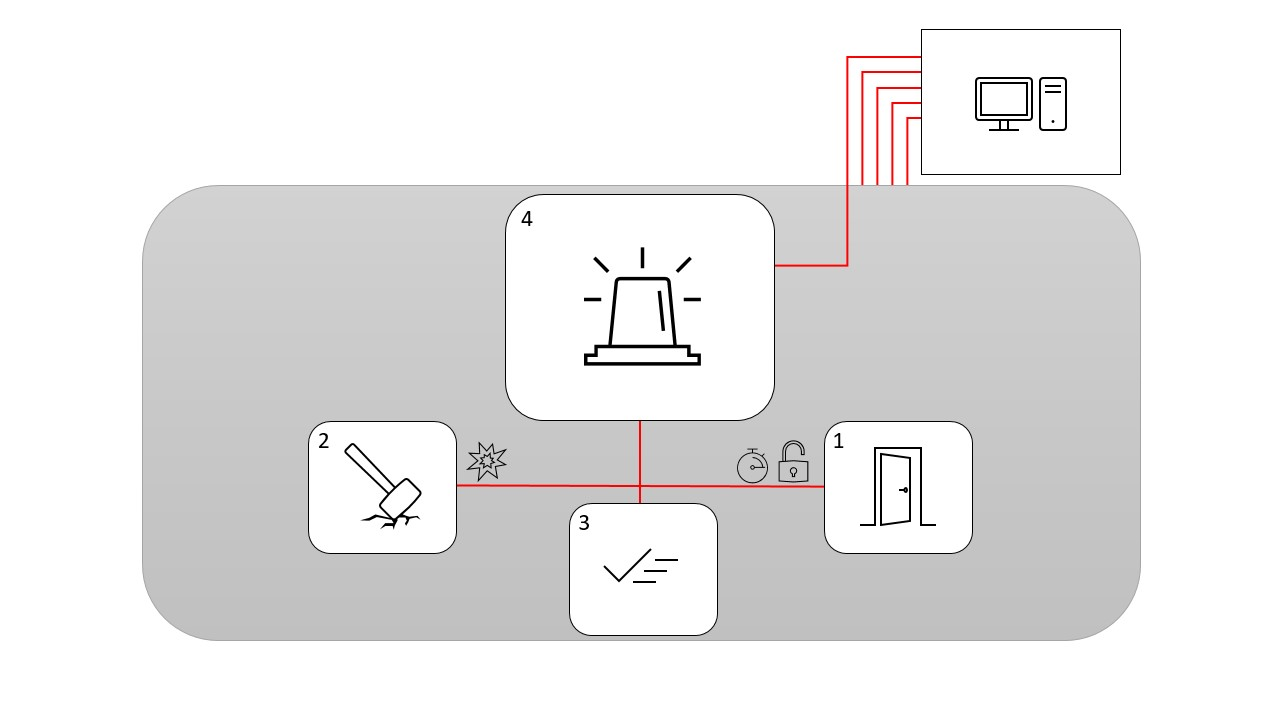
\includegraphics[width=\textwidth]{system3.jpg}
